%!TEX root = ../dokumentation.tex

\chapter{Grundlagen}

\section{JavaScript}

\subsection{Der Sprachstandard ECMAScript}
ECMAScript spezifiziert den Sprachstandard von JavaScript. Dieser wird seit dem Jahr 1997 Jahren von der European Computer Manufactures Association (kurz: ECMA) weiterentwickelt. Zunächst wurden die Versionen durchnummeriert (ES1, ES2, ES3, ES4, und ES5). Im Jahre 2015 wurde beschlossen, dass jährlich eine neue Version von ECMAScript erscheinen soll. Daher tragen die nachfolgenden Versionen das Veröffentlichungsjahr im Namen (ECMAScript2015, ECMAScript2016, ECMAScript2017, ECMAScript2018, …). 

Die neusten Browser unterstützen meist den aktuellsten ECMAScript Sprachstandard. Allerdings verwendet nicht jeder Benutzer einen neuen Browser. Um die Kompatibilität einer Webanwendung zu gewährleisten, muss der Code in eine niedrigere von den meisten Browsern unterstütze Version transpiliert werden.\autocites[vgl.][27\psqq]{Woiwode.2018}[vgl.][]{Terlson.2018}[vgl.][13\psqq]{Steyer.2017}

In ECMAScript2015 wurden die Variablentypen let zur Eingrenzung des Geltungsbereichs einer Variable und const zur Deklaration einer Konstanten eingeführt. Zudem können seit ECMAScript2015 auch Klassen und Module in JavaScript definiert werden. Eine Klasse kann mehrere Eigenschaften und Methoden enthalten. Zudem können Klassen voneinander erben.

Jede Datei ist ein eigenes Modul. Module fassen zusammengehörige Codeeinheiten zusammen und können Interfaces, Klassen oder Variablen bereitstellen, die wiederum von anderen Modulen verwendet werden können.\autocites[vgl.][34\psq]{Woiwode.2018}[vgl.][19\psqq]{Steyer.2017}

Seit ECMAScript2017 können Dekoratoren für die Angabe von Metainformationen zu einer Klasse verwendet werden. Dies wird beispielsweise von Angular zur Kennzeichnung und Konfiguration der unterschiedlichen Bestandteile des Frameworks verwendet.\autocites[vgl.][30\psqq]{Woiwode.2018}

\comment{Grafik ersetzen!}
\begin{figure}[h]
	\centering
	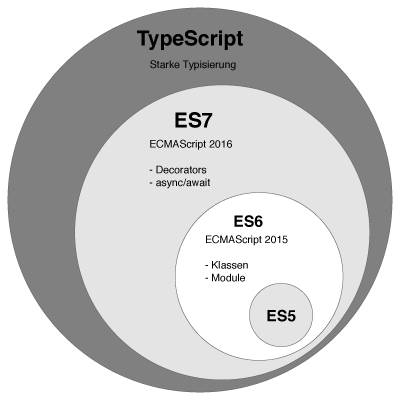
\includegraphics[width=0.5\linewidth]{JavaScript.png}
	\caption{Beziehung zwischen ECMAScript und TypeScript} 
	\quelle{\textcite[28]{Woiwode.2018}}
	\label{fig:ECMAScript}
\end{figure}

\subsection{Die Obermenge TypeScript}
TypeScript ist eine von Anders Hejlsberg bei Microsoft entwickelte Sprache. Diese erweitert die bestehende ECMAScript Version um weitere Sprachelemente und bildet somit eine Obermenge von JavaScript (siehe \autoref{fig:ECMAScript}). TypeScript ergänzt JavaScript unter anderem um ein stärkeres Typsystem. Hierdurch können Typfehler bereits zur Compilezeit erkannt und Tools zur Codeanalyse (automatische Codevervollständigung, Refactoring-Unterstützung, …) eingesetzt werden.\autocites[vgl.][27\psqq]{Woiwode.2018}[vgl.][13\psqq]{Steyer.2017}[vgl.][10]{Zeigermann.2016}

Folgende Basistypen stellt TypeScript zur Verfügung: \autocite[vgl.][34\psqq]{Woiwode.2018}
\begin{description}
	\item [number]  Ganz- oder Kommazahl
	\item [string] Zeichenkette
	\item [boolean] Wahrheitswert 
	\item [Array<typ>] typisierte Arrays
	\item [any] beliebiger Datentyp
\end{description}

TypeScript ermöglicht die Verwendung von Interfaces. \autocites[vgl.][40\psq]{Woiwode.2018}

\subsection{Die Erweiterung JSX}
Die Spracherweiterung JSX ermöglicht die Verwendung einer HTML ähnlichen Syntax in JavaScript. JSX wird durch einen geeigneten Transpilierer in gültiges JavaScript übersetzt. 


Die Spracherweiterung kann zum Beispiel bei der Verwendung des Frameworks React eingesetzt werden. Dieses Framework verwendet zur Darstellung der Benutzeroberfläche keine Templates. Die Benutzeroberfläche wird stattdessen mit JavaScript Befehlen aufgebaut. Um dies zu erleichtern, kann JSX verwendet werden. \autocites[vgl.][59\psqq]{Zeigermann.2016}[vgl.][65]{Stefanov.2017}



\comment{NodeJS}
